\chapter{弱场、引力波与作用量原理}

广义相对论的精确方程是非线性的，在尚未解决任何一个物理问题之前，其分量形式就可能变得极其繁复。作为本课程的最后一讲，最好把原理与记账分开。我们将追问：当引力场微弱时，爱因斯坦方程会变成什么？辨认出该近似中所包含的波，最后再看完整的场方程如何纳入一个极为紧凑的作用量原理之中。

有三个问题组织起这场讨论。弱引力场意味着什么？为什么精确理论是非线性的，而弱场理论却是线性的？又有哪些物理效应能把引力波与单纯的坐标抖动区分开来？

\section{平衡几何的微小扰动}

“弱”是一种近似方案。若一个无量纲扰动的量级为\(\epsilon\ll1\)，则其平方的量级为\(\epsilon^2\)，而一阶计算会一致地舍弃后者。熟悉的例子是围绕平衡位置作小振动的力学系统。其精确方程可能是非线性的，但足够小的振动服从线性方程。

对于引力，平衡背景将取空的平直时空。从爱因斯坦真空方程出发，
\begin{equation}
 R_{\mu\nu}-\frac12 g_{\mu\nu}R=0.
 \label{eq:l10-vacuum-einstein}
\end{equation}
在四维中取迹给出
\begin{equation}
 g^{\mu\nu}
 \left(R_{\mu\nu}-\frac12 g_{\mu\nu}R\right)
 =R-2R=-R=0,
\end{equation}
因此真空方程等价于
\begin{equation}
 R_{\mu\nu}=0.
 \label{eq:l10-ricci-flat}
\end{equation}

\begin{figure}[htbp]
\centering
\includegraphics[width=0.68\textwidth]{lecture_10_figure_02.png}
\caption{真空方程\(R_{\mu\nu}=0\)，在弱场论证的开头被单独列出。}
\lectureframe{00:03:11}
\end{figure}

这里，平衡指的是无源且不依赖于时间的解。平直时空是最简单的此类解。有一点限定至关重要：平直并不意味着度规的分量在每一个坐标系中都等于某个特定的矩阵。它意味着可以选取惯性坐标，使得
\begin{equation}
 g_{\mu\nu}=\eta_{\mu\nu}.
\end{equation}
几何与用来描述它的坐标之间的这一区分，很快就会成为核心的微妙之处。

现在设想一个剧烈的源，例如一个致密双星。它的近场可能很强，但在远离源处，扰动向外传播并变得很小。在合适的坐标系中，度规于是可以写成
\begin{equation}
 g_{\mu\nu}(x)=\eta_{\mu\nu}+h_{\mu\nu}(x),
 \qquad |h_{\mu\nu}|\ll1.
 \label{eq:weak-split}
\end{equation}
扰动\(h_{\mu\nu}\)允许依赖于全部四个时空坐标。微弱意味着高于一次的幂将被忽略。

\section{一阶下幸存的部分}

完整的里奇张量太长，在此阶段没有用处。它的结构就足够了。克里斯托费尔符号包含一个逆度规和度规的一次导数，而曲率则包含一个克里斯托费尔符号的导数以及两个克里斯托费尔符号的乘积：
\begin{equation}
 \Gamma\sim\frac12 g^{-1}\partial g,
 \qquad
 R\sim\partial\Gamma+\Gamma\Gamma.
 \label{eq:curvature-skeleton}
\end{equation}

\begin{figure}[htbp]
\centering
\includegraphics[width=0.84\textwidth]{lecture_10_figure_03.png}
\caption{弱场拆分与示意性构造\(R\sim\partial\Gamma+\Gamma\Gamma\)。该记号揭示了\(h\)的各阶，而无需展开每一个指标。}
\lectureframe{00:10:17}
\end{figure}

逆度规由
\(g^{\mu\alpha}g_{\alpha\nu}=\delta^\mu{}_\nu\)给出。到一阶，
\begin{equation}
 g^{\mu\nu}=\eta^{\mu\nu}-h^{\mu\nu}+O(h^2),
 \label{eq:inverse-weak}
\end{equation}
其中\(h\)上的指标用背景度规升降。在惯性坐标中背景是常数，
\begin{equation}
 \partial_\alpha\eta_{\mu\nu}=0,
\end{equation}
因此
\begin{equation}
 \partial_\alpha g_{\mu\nu}
 =\partial_\alpha h_{\mu\nu}.
\end{equation}
从而，
\begin{equation}
\begin{aligned}
 \Gamma&=O(\partial h),\\
 R_{\mu\nu}
 &=O(\partial\partial h)+O\bigl((\partial h)^2\bigr)\\
 &\quad+O(h\,\partial\partial h).
\end{aligned}
 \label{eq:ricci-orders}
\end{equation}

\begin{figure}[htbp]
\centering
\includegraphics[width=0.84\textwidth]{lecture_10_figure_04.png}
\caption{黑板上对逆度规的展开，以及\(\partial\eta=0\)这一观察。在领头阶只剩下\(h_{\mu\nu}\)的导数。}
\lectureframe{00:11:55}
\end{figure}

方程~\eqref{eq:ricci-orders}中的最后两项对扰动是二次的，因而被略去。因此真空方程是涉及\(h_{\mu\nu}\)二阶导数的线性方程。这就是线性化的全部含义。它并不是断言爱因斯坦的精确理论是线性的。

\begin{classroomqa}
\audiencequestion{曲率张量有四个指标，而里奇张量有两个。如果两个导数已经带有指标，而\(h_{\mu\nu}\)又带有两个指标，那么指标计数如何成立？}
\lecturerresponse{里奇张量是通过对曲率张量中的一对指标作缩并得到的。该缩并所用的度规留下两个自由指标，恰好就是\(R_{\mu\nu}\)所带的那一对。符号形式\(\partial\partial h\)掩盖了这些缩并；它是一个阶数计数，而不是完整的带指标公式。
\lecturetimestamp{00:18:45--00:19:53}}
\end{classroomqa}

\begin{classroomqa}
\audiencequestion{用逆度规作缩并是否会引入诸如\(h\,\partial^2h\)这样的项，如果是，为什么可以忽略它们？}
\lecturerresponse{确实会。把\(g^{-1}\)替换为
\(\eta^{-1}-h+\cdots\)会同时产生线性项
\(\eta^{-1}\partial^2h\)以及含有第二个\(h\)的修正项。后者是二次的。同一条规则也舍弃
\(h\,\partial h\)、\(h\,\partial^2h\)和
\((\partial h)^2\)。只保留扰动的一次幂，正是这里所作的近似。
\lecturetimestamp{00:19:55--00:21:14}}
\end{classroomqa}

\section{为什么方程看起来像波}

二阶导数的场方程自然暗示了波的传播。对于一个沿\(z\)轴运动的标量函数，原型是
\begin{equation}
 \left(\partial_t^2-\partial_z^2\right)\phi=0,
\end{equation}
其解包括任意向右和向左运动的剖面，
\begin{equation}
 \phi(z,t)=f(z-t)+g(z+t).
\end{equation}
在三个空间维度中，同一方程是
\begin{equation}
 \left(\partial_t^2-\nabla^2\right)\phi=0.
\end{equation}
它的线性性质允许叠加：两个解之和仍是解。

引力不是标量场。微扰具有张量分量，而方程\(R_{\mu\nu}=0\)最初似乎提供了许多分量方程。它们并非全部独立；有些是约束，有些反映了坐标自由度。这与麦克斯韦理论类似，在那里一族场方程最终只留下物理的横波。

在施加适当的坐标条件后，辐射分量服从普通的波动方程，
\begin{equation}
 \Box h_{\mu\nu}=0,
 \qquad
 \Box=\eta^{\alpha\beta}\partial_\alpha\partial_\beta.
 \label{eq:linear-wave}
\end{equation}
\(\Box\)内部的精确符号取决于号差约定；其内容则不依赖于此。扰动在光锥上传播。

\section{坐标抖动不是引力波}

在把线性化方程的每个解都接受为物理波之前，我们必须回到坐标的告诫。平直空间可以用弯曲的坐标线来描述。于是它的度规分量不同于笛卡尔值，尽管其曲率仍然为零。

黑板本身就提供了例子。在其平坦表面上画出直的笛卡尔坐标并写出
\begin{equation}
 ds^2=\delta_{mn}\,dx'^m dx'^n.
\end{equation}
现在用略微抖动的坐标重新标记同样的点，
\begin{equation}
 x'^m=x^m+f^m(x).
 \label{eq:small-coordinate-change}
\end{equation}
微分变为
\begin{equation}
 dx'^m=dx^m+\partial_n f^m\,dx^n.
\end{equation}
代入线元并只保留\(f\)的一阶项，得到
\begin{align}
 ds^2
 &=\delta_{mn}dx^m dx^n\\
 &\quad+\left(\partial_m f_n+\partial_n f_m\right)dx^m dx^n
 +O(f^2).
\end{align}
因此，形如
\begin{equation}
 h_{mn}=\partial_m f_n+\partial_n f_m
 \label{eq:pure-gauge}
\end{equation}
的表观微扰根本不能描述任何新几何。它只是抖动坐标下的平直空间。

\begin{figure}[htbp]
\centering
\includegraphics[width=0.84\textwidth]{lecture_10_figure_05.png}
\caption{黑板上的坐标抖动计算。一次小的重新坐标化诱导出一个看起来很小的\(h_{mn}\)，尽管黑板仍然是平坦的。}
\lectureframe{00:27:54}
\end{figure}

方程~\eqref{eq:pure-gauge}是坐标自由度即规范自由度的线性化形式。需要附加条件来消除这些虚假的微扰。详细的规范代数不在此展开。其作用才是要点：它去除描述的变化，同时保留曲率的变化。一旦坐标自由度和约束方程都被考虑在内，物理内容就归结为两个独立的波偏振。

\begin{figure}[htbp]
\centering
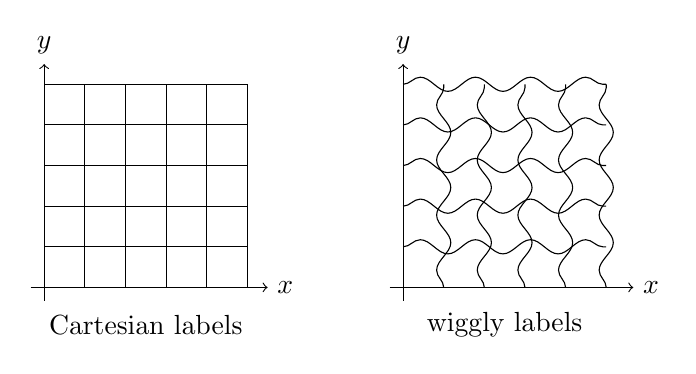
\begin{tikzpicture}[scale=0.86]
\begin{scope}
\draw[->] (-0.2,0) -- (3.3,0) node[right] {$x$};
\draw[->] (0,-0.2) -- (0,3.3) node[above] {$y$};
\foreach \u in {0.6,1.2,1.8,2.4,3.0}{
  \draw (\u,0) -- (\u,3.0);
  \draw (0,\u) -- (3.0,\u);
}
\node at (1.5,-0.55) {Cartesian labels};
\end{scope}
\begin{scope}[xshift=5.3cm]
\draw[->] (-0.2,0) -- (3.4,0) node[right] {$x$};
\draw[->] (0,-0.2) -- (0,3.3) node[above] {$y$};
\foreach \u in {0.6,1.2,1.8,2.4,3.0}{
  \draw[decorate,decoration={snake,amplitude=0.09cm,segment length=0.7cm}]
    (\u,0) -- (\u,3.0);
  \draw[decorate,decoration={snake,amplitude=0.09cm,segment length=0.7cm}]
    (0,\u) -- (3.0,\u);
}
\node at (1.5,-0.55) {wiggly labels};
\end{scope}
\end{tikzpicture}
\caption{几何保持平坦，而坐标网格发生变化。仅凭度规分量无法判断一个微扰是否是物理的。}
\end{figure}

\section{沿z轴传播的波}

选择一列沿\(z\)正方向传播的平面波。其相位可以写成
\begin{equation}
 k(z-t),
\end{equation}
因此一个代表性分量具有形式
\begin{equation}
 h_{\mu\nu}(z,t)
 =h_{\mu\nu}^{(0)}\sin k(z-t).
 \label{eq:plane-wave}
\end{equation}
等相位面满足\(z-t=\text{constant}\)；因此传播速度就是光速。

在横向无迹描述中，含时间指标或\(z\)指标的分量消失：
\begin{equation}
 h_{0\mu}=0,
 \qquad
 h_{z\mu}=0.
 \label{eq:tt-transverse}
\end{equation}
只剩下\(x\)-\(y\)块。它是对称且无迹的，
\begin{equation}
 h_{xy}=h_{yx},
 \qquad
 h_{xx}+h_{yy}=0.
 \label{eq:tt-trace}
\end{equation}

\begin{figure}[htbp]
\centering
\includegraphics[width=0.84\textwidth]{lecture_10_figure_06.png}
\caption{沿\(z\)传播的波，表示为横向平面的堆叠。存留的\(x\)-\(y\)振幅满足\(h_{xx}+h_{yy}=0\)。}
\lectureframe{00:43:36}
\end{figure}

因此存在两个独立的模式。对于\(i,j\in\{x,y\}\)，它们可以表示为
\begin{equation}
 h^{\mathrm{TT}}_{ij}(z,t)
 =
 \begin{pmatrix}
 h_+ & h_\times\\
 h_\times & -h_+
 \end{pmatrix}
 \sin k(z-t).
 \label{eq:polarization-matrix}
\end{equation}
对角模式称为加偏振。非对角模式称为叉偏振。将横向轴旋转\(45^\circ\)会使一个模式变为另一个，而任意线偏振波都是两者的叠加。在这个理论中没有进一步的独立偏振。

\begin{figure}[htbp]
\centering
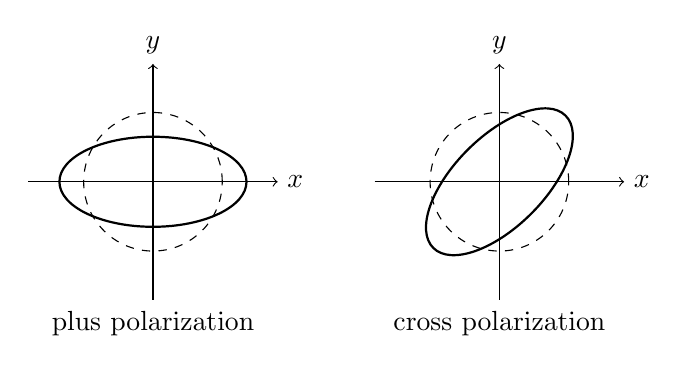
\begin{tikzpicture}[scale=0.88]
\begin{scope}
\draw[->] (-1.8,0) -- (1.8,0) node[right] {$x$};
\draw[->] (0,-1.7) -- (0,1.7) node[above] {$y$};
\draw[dashed] (0,0) circle (1.0);
\draw[thick] (0,0) ellipse (1.35 and 0.65);
\node at (0,-2.05) {plus polarization};
\end{scope}
\begin{scope}[xshift=5.0cm]
\draw[->] (-1.8,0) -- (1.8,0) node[right] {$x$};
\draw[->] (0,-1.7) -- (0,1.7) node[above] {$y$};
\draw[dashed] (0,0) circle (1.0);
\draw[thick,rotate=45] (0,0) ellipse (1.35 and 0.65);
\node at (0,-2.05) {cross polarization};
\end{scope}
\end{tikzpicture}
\caption{半个周期拉伸一个横向方向，同时挤压垂直方向。再过半个周期，形变反转。}
\end{figure}

\section{从度规分量到物理应变}

固定\(z\)和\(t\)并考察横向平面。对于纯加波，
\begin{equation}
 ds_\perp^2
 =(1+h_{xx})\,dx^2+(1-h_{xx})\,dy^2.
 \label{eq:transverse-distance}
\end{equation}
当\(h_{xx}>0\)时，\(x\)方向上一个固定的坐标间隔具有稍大的固有长度，而相应的\(y\)间隔具有稍小的固有长度。半个周期后\(h_{xx}\)改变符号，角色互换。一个正方形交替地水平拉伸、竖直挤压，然后水平挤压、竖直拉伸。对于叉偏振，同样的交替发生在旋转了\(45^\circ\)的轴上。

在一阶近似下，初始长度为\(L\)的臂变化为
\begin{equation}
 \frac{\Delta L}{L}\simeq\frac12 h_{ij}n^i n^j,
 \label{eq:fractional-strain}
\end{equation}
其中\(\mathbf n\)沿臂的方向。这个公式将度规扰动转化为探测器测得的无量纲应变。

\begin{classroomqa}
\audiencequestion{米尺是靠电磁力结合在一起的，并不会简单地随坐标改变其静止长度。那么，图景是否应该改用自由分离的检验质量？}
\lecturerresponse{这一区别很重要。真实的杆具有弹性，因此潮汐场会在其内部驱动应力；钢杆和木杆一般会以不同的量作出响应。自由悬挂的检验质量避免了那种特定的弹性响应，更直接地揭示相对加速度。无论哪种情况，经过的波都不仅仅是在重新标记各点。它随时间变化的曲率产生物理效应。
\lecturetimestamp{00:47:23--00:48:48}}
\end{classroomqa}

精确的局域陈述是测地偏离。对于相隔\(\xi^i\)的邻近自由下落粒子，
\begin{equation}
 \frac{d^2\xi^i}{dt^2}
 =-R^i{}_{0j0}\,\xi^j.
 \label{eq:geodesic-deviation}
\end{equation}
在弱的横向无迹波中，
\begin{equation}
 R_{0i0j}=-\frac12\ddot h^{\mathrm{TT}}_{ij},
 \label{eq:tidal-curvature}
\end{equation}
因此振荡的度规产生交替的潮汐加速度。这就是为什么随时间变化的波不能被当作对尺子的静态选择而加以摒弃。它具有非零曲率。

\begin{classroomqa}
\audiencequestion{如果该区域内每一把尺子都受到影响，那还能用什么来测量这种挤压和拉伸？}
\lecturerresponse{应变计可以记录材料物体中感生的真实应力。更好的做法是，可以监测自由悬挂质量之间不断变化的间距。静态、均匀的重新标度可以被吸收进测量装置中，但振荡的曲率会驱动一种能够被记录下来的响应。
\lecturetimestamp{00:51:10--00:52:02}}
\end{classroomqa}

\section{源与探测器}

电磁波由运动的电荷和电流产生。引力波由运动的质能和能量分布产生。能量守恒和动量守恒排除了孤立系统的引力单极辐射和偶极辐射，因此主导的辐射矩是四极矩。一个致密双星恰好提供了所需的、不断变化的四极矩：两个致密天体相互绕转，并向远场发射波。

在双星附近，时空弯曲强烈，方程~\eqref{eq:weak-split}的线性展开不可靠。在远处，出射波散布到更大的面积上，其振幅变得很小，线性化描述变得准确。对于位于距源\(z\)轴上的观测者，可测量的拉伸位于横向的\(x\)-\(y\)平面内。

\begin{classroomqa}
\audiencequestion{图中画的尺子是抽象的坐标尺，还是物理的米尺？一把可变的尺子又如何能测量这种效应？}
\lecturerresponse{它可以是物理物体，但那样一来它的材料属性就很重要。曲率提供潮汐应力；钢和木在其作用下不必以相同方式形变。比较它们的响应本身就已经是一种测量。更干净的探测器用分离的检验质量取代杆，并测量它们的差异运动。
\lecturetimestamp{00:54:00--00:55:19}}
\end{classroomqa}

共振探测器是一种策略。如果一个机械系统的固有频率接近入射波的频率，波就会相干地驱动它并放大响应。干涉仪采用另一种策略：反射镜充当检验质量，激光干涉比较垂直臂的有效长度。一个加偏振的波使一条臂变长，同时使另一条臂变短，而这正是一台干涉仪被设计来探测的差异信号。

\begin{classroomqa}
\audiencequestion{这会成为引力波探测器的基础吗？}
\lecturerresponse{是的。坚硬的杆几乎不变，而自由悬挂的端部质量可以发生相对加速度。人们还可以利用共振，使微弱的周期性驱动产生更大的响应。预期的天体物理应变极其微小，量级为\(10^{-21}\)，因此探测器设计就是把那微小的差异运动转化为可测量信号的艺术。
\lecturetimestamp{00:55:20--00:57:10}}
\end{classroomqa}

\begin{classroomqa}
\audiencequestion{LIGO是这种探测器的一个例子吗？}
\lecturerresponse{是的。它的基本观测量来自在垂直臂中反射镜之间来回反射的激光。引力波改变相对光程长度，从而改变干涉图样。在这次讲座之时，该仪器尚未做出直接探测；那一历史状况后来改变了。\editorialnote{首次直接观测，GW150914，记录于2015年，并于2016年宣布。}
\lecturetimestamp{00:57:16--00:58:05}}
\end{classroomqa}

\begin{classroomqa}
\audiencequestion{波解给出的传播速率是多少？}
\lecturerresponse{光速。相位 \(k(z-t)\) 在 \(z\) 中移动一个单位，在 \(t\) 中也移动一个单位，而线性化爱因斯坦方程与电磁波方程具有相同的光锥传播结构。
\lecturetimestamp{00:58:07--00:58:16}}
\end{classroomqa}

黑洞碰撞与致密双星是特别有前景的源。在碰撞附近，引力场强烈非线性，释放能量中相当大的一部分可能以引力辐射的形式离开。当信号到达远处探测器时，其振幅已足够弱，以至于线性波传播是极好的描述。因此，引力辐射开启了一条不必依赖发射光的天文观测通道。

\section{双脉冲星与间接证据}

辐射携带能量。如果双星系统发射引力波，轨道能量就会减少，天体缓慢向内旋进，轨道周期随之改变。双脉冲星提供了一座足够精确的时钟来测量这一变化。其观测到的轨道演化与广义相对论预言的能量损失在定量上一致。

在讲座所处的历史背景下，这就是决定性的间接证据：当时还没有任何探测器记录到穿过地球的波，但轨道正以引力辐射所要求的速率损失能量。这些波已经可以通过它们对自身源所造成的影响而被观测到。

\begin{classroomqa}
\audiencequestion{最初的脉冲双星系统以什么频率或周期为特征？是在毫秒尺度上吗？}
\lecturerresponse{毫秒尺度指的是脉冲星的自转，而不是两颗星的轨道。课堂上核对了该数值，发现轨道周期约为 \(7.75\) 小时。这一区分很重要：引力辐射追踪的是双星轨道运动，而射电脉冲则提供了用来跟踪它的精确时钟。
\lecturetimestamp{01:01:27--01:03:28}}
\end{classroomqa}

\begin{classroomqa}
\audiencequestion{在数十年的观测中，累积的轨道计时变化了多少？}
\lecturerresponse{所引用的累积偏移约为三十秒。瞬时相对变化极小，但数十年精确的脉冲计时使累积效应变得可见。
\lecturetimestamp{01:03:34--01:03:54}}
\end{classroomqa}

\section{时间依赖、曲率与线性的限度}

\begin{classroomqa}
\audiencequestion{为什么选择横向的 \(x\)-\(y\) 平面？如果改为考虑涉及 \(x\) 和 \(t\) 的平面，会发生什么？}
\lecturerresponse{波本身同时依赖于 \(z\) 和 \(t\)，但横向指的是垂直于其空间传播方向的空间方向。对于沿 \(z\) 传播的波，物理度规振幅可以选在 \(x\)-\(y\) 块中。其他表观分量要么不存在，要么是可移除的坐标抖动。
\lecturetimestamp{01:02:22--01:03:17}}
\end{classroomqa}

\begin{classroomqa}
\audiencequestion{时间本身在振荡吗？}
\lecturerresponse{不是。波作为时间的函数而振荡。在固定空间位置上，分量 \(h_{ij}(z,t)\) 周期性地变化。时间只是场所依赖的一个坐标，而不是在这幅图像中被交替拉伸和压缩的对象。
\lecturetimestamp{01:04:00--01:04:18}}
\end{classroomqa}

\begin{classroomqa}
\audiencequestion{如果所有 \(h_{0\mu}\) 都为零，是否就不存在涉及时间方向的曲率？}
\lecturerresponse{存在。存活下来的空间分量依赖于时间，而曲率包含它们的二阶导数。因此，诸如 \(\partial_t^2h_{ij}\) 这样的导数会产生分量 \(R_{0i0j}\)。\(h_{\mu\nu}\) 的时间指标分量为零，并不意味着依赖于时间的曲率为零。
\lecturetimestamp{01:05:15--01:06:09}}
\end{classroomqa}

线性波动方程之所以出现，是因为假定 \(h\) 很小，而不是因为移除了坐标假象。这是两种不同的操作。规范固定识别出物理自由度；线性化则丢弃非线性相互作用。

\begin{classroomqa}
\audiencequestion{爱因斯坦方程是非线性的，但由此得到的波动方程却是线性的。这种线性是由消除非物理解造成的吗？}
\lecturerresponse{不是。它是由小振幅近似造成的。含有 \(h\) 的二次幂的项被丢弃了。移除坐标抖动决定哪些解是物理的；这并不是使方程线性的原因。
\lecturetimestamp{01:06:45--01:07:29}}
\end{classroomqa}

\begin{classroomqa}
\audiencequestion{求解线性化方程后，与精确解相比误差有多大？}
\lecturerresponse{最先被忽略的修正项为 \(h^2\) 阶。若 \(h\sim10^{-1}\)，它们为 \(10^{-2}\) 阶；若 \(h\sim10^{-3}\)，它们为 \(10^{-6}\) 阶。微扰计算之后必须始终加以检验，以确保所假设的小参数确实很小。
\lecturetimestamp{01:07:35--01:08:31}}
\end{classroomqa}

\begin{classroomqa}
\audiencequestion{当高阶项变得重要时，波会失去其横向特性吗？}
\lecturerresponse{本质的横向辐射特性仍然保留，但线性叠加不再成立。强波与由其他波携带的引力场相互作用；它们不再彼此不变地穿过，而是发生散射。
\lecturetimestamp{01:08:34--01:09:11}}
\end{classroomqa}

\begin{classroomqa}
\audiencequestion{机械波的速度取决于刚度和密度。是否存在一种可类比的意义，使时空也具有刚度？}
\lecturerresponse{仅作为一种类比。对于物质介质，传播取决于诸如刚度除以密度这样的组合。由于电磁波和引力波以 \(c\) 传播，旧的机械语言会称它们的介质极其刚硬。现代物理学并不为时空赋予普通的杨氏模量；不变的事实是由场方程所固定的光速传播。
\lecturetimestamp{01:09:12--01:11:10}}
\end{classroomqa}

\section{第二条路径：驻定作用量}

波动的讨论既已完成，还有时间做最后一次视角的转换。驻定作用量原理是经典力学、电磁学、场论和标准模型的共同语言。广义相对论属于同一结构。

对于粒子，作用量是沿轨迹的积分。对于场，一个历史为时空的每一点赋予一个场值 \(\phi(x)\)，而作用量是时空上的积分：
\begin{equation}
 S[\phi]
 =\int d^4x\,
 \mathcal L\bigl(\phi,\partial_\mu\phi\bigr).
 \label{eq:field-action}
\end{equation}
每一个足够规则的 \(\phi(x)\) 都是一个可能的历史，正如每一条足够规则的路径都是一条可能的粒子轨迹，但大多数并不是解。物理的历史是在固定边界数据下作用量的驻定点：
\begin{equation}
 \delta S=0.
 \label{eq:stationary-action}
\end{equation}
对于场，边界包围的是一个时空区域，而不仅仅是指定一条路径的两个端点。随后，欧拉--拉格朗日方程选出在给定边界值之间的插值。

爱因斯坦场方程可以完全以这种方式得到。变分很长，但作用量本身很简单。在写出它之前，我们需要时空体积的恰当测度。

\section{为什么行列式度量体积}

从二维的对角度规开始，
\begin{equation}
 ds^2=g_{xx}\,dx^2+g_{yy}\,dy^2.
\end{equation}
一个边长为 \(dx\) 和 \(dy\) 的坐标矩形，其固有边长分别为 \(\sqrt{g_{xx}}\,dx\) 和 \(\sqrt{g_{yy}}\,dy\)，因此其固有面积为
\begin{equation}
 dA
 =\sqrt{g_{xx}g_{yy}}\,dx\,dy.
\end{equation}
如果存在非对角分量 \(g_{xy}\)，坐标边就不必正交。修正后的面积为
\begin{equation}
 dA
 =\sqrt{g_{xx}g_{yy}-g_{xy}^2}\,dx\,dy
 =\sqrt{\det g}\,dx\,dy.
 \label{eq:area-determinant}
\end{equation}

\begin{figure}[htbp]
\centering
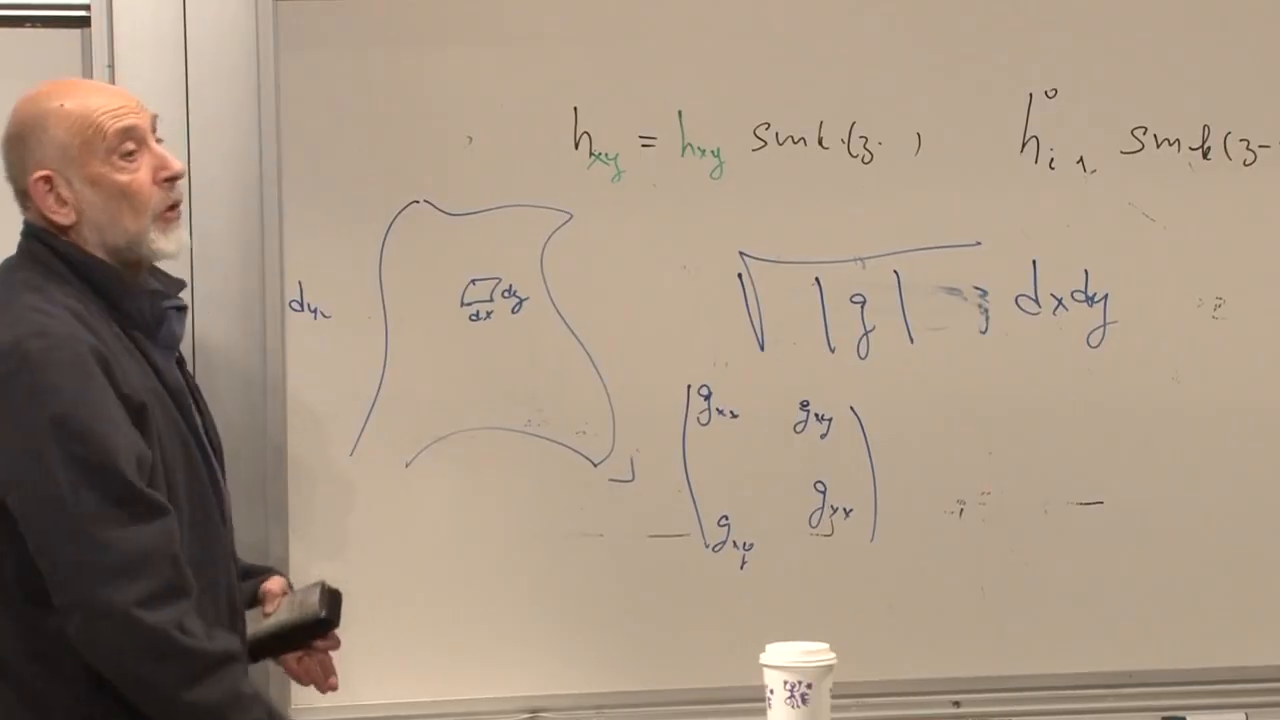
\includegraphics[width=0.84\textwidth]{lecture_10_figure_07.png}
\caption{从小的坐标矩形到固有面积元 \(\sqrt{\lvert g\rvert}\,dx\,dy\) 的推广。行列式同时包含了两个对角长度和非对角剪切。}
\lectureframe{01:21:25}
\end{figure}

同样的构造在任何维度都适用：
\begin{equation}
 dV_n=\sqrt{|\det g|}\,d^nx.
\end{equation}
对于洛伦兹时空，若 \(g=\det(g_{\mu\nu})\)，不变的四维体积元按惯例写作
\begin{equation}
 dV_4=\sqrt{|g|}\,d^4x,
 \label{eq:four-volume}
\end{equation}
或在 mostly-plus 约定下写作 \(\sqrt{-g}\,d^4x\)。一个区域的坐标可以改变，但其物理四维体积不变。

将此测度乘以任意标量 \(F(x)\) 并积分，就产生一个坐标不变量：
\begin{equation}
 \int d^4x\,\sqrt{|g|}\,F(x).
 \label{eq:invariant-scalar-integral}
\end{equation}
一个广义协变理论的作用量应当具有这种形式。否则，由它导出的场方程可能依赖于坐标的任意选择。

\section{爱因斯坦--希尔伯特作用量}

对于纯引力，动力学场就是度规本身。由度规及其前两阶导数构成的最简单的非常数标量是标量曲率 \(R\)。常数也是标量；其系数就是宇宙学常数。在符号约定和边界项的意义上，引力作用量的标准归一化为
\begin{equation}
 S_{\mathrm{grav}}
 =
 \frac{1}{16\pi G}
 \int d^4x\,\sqrt{|g|}\,(R-2\Lambda).
 \label{eq:einstein-hilbert}
\end{equation}

\begin{figure}[htbp]
\centering
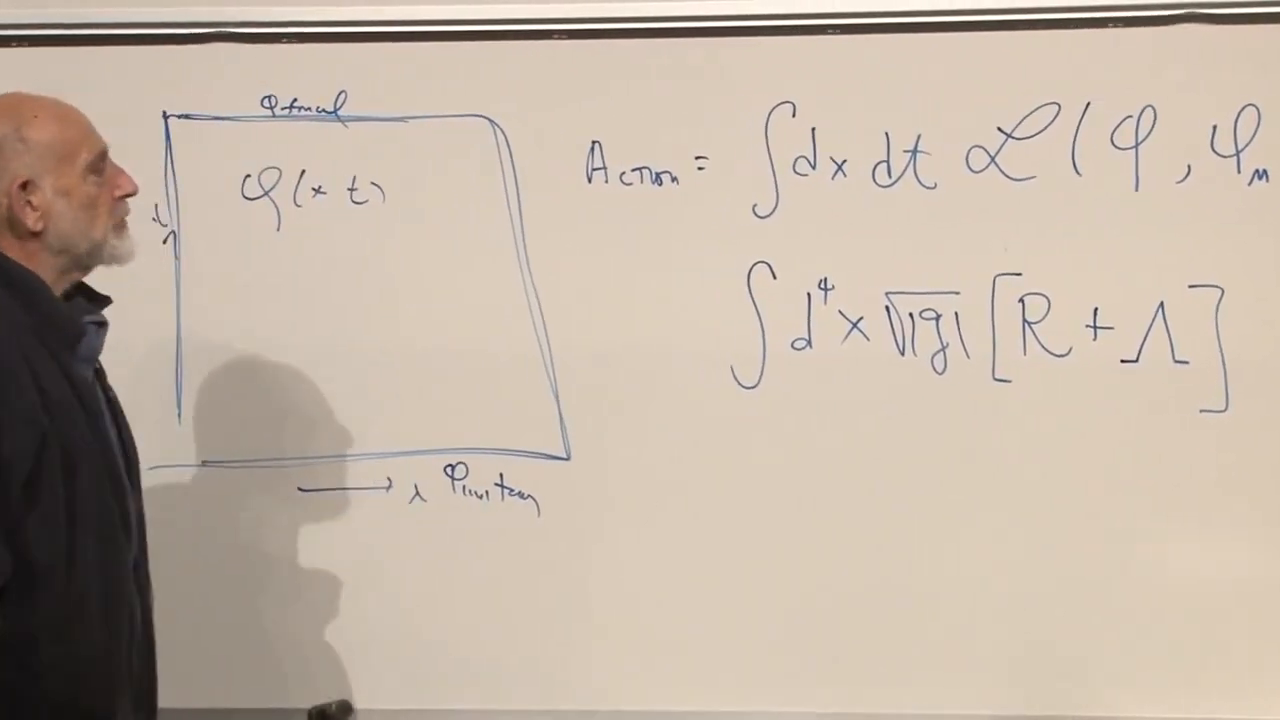
\includegraphics[width=0.84\textwidth]{lecture_10_figure_08.png}
\caption{场的历史图像与引力作用量。标量曲率提供动力学；常数项正比于时空体积。}
\lectureframe{01:26:32}
\end{figure}

正比于 \(\Lambda\) 的项只是总时空体积的倍数。先前的波动方程是在 \(\Lambda=0\) 的真空中导出的，因此该项在那里没有出现。

物质通过物质作用量加入，
\begin{equation}
 S=S_{\mathrm{grav}}+S_{\mathrm{matter}}.
\end{equation}
例如，对于电磁学，不变场贡献由反对称张量\(F_{\mu\nu}\)构建：
\begin{equation}
 S_{\mathrm{EM}}
 =-\frac14
 \int d^4x\,\sqrt{|g|}\,
 F_{\mu\nu}F^{\mu\nu}.
\end{equation}
对总作用量关于逆度规变分，定义了应力-能量张量，并给出
\begin{equation}
 R_{\mu\nu}
 -\frac12 g_{\mu\nu}R
 +\Lambda g_{\mu\nu}
 =8\pi G\,T_{\mu\nu}.
 \label{eq:einstein-from-action}
\end{equation}
因此，这个紧凑的作用量包含了完整的场方程。在真空中，当\(\Lambda=0\)时，它约化为先前研究引力波时所依据的理论。

\begin{classroomqa}
\audiencequestion{应力-能量张量在哪里进入作用量原理？}
\lecturerresponse{它来自描述物质和其他场的附加项。电磁能量、粒子场以及任何其他物质内容都对\(S_{\mathrm{matter}}\)有贡献。它们的度规变分给出\(T_{\mu\nu}\)。只包含\(\sqrt{|g|}R\)的积分就是真空引力理论。
\lecturetimestamp{01:27:26--01:28:25}}
\end{classroomqa}

推导在概念上直截了当，在代数上却令人不快。人们从度规构造克里斯托费尔符号，构造曲率，缩并形成\(R\)，乘以行列式因子，并对所得表达式变分。讲座开玩笑说，这个练习应该花五分钟，做不出来就意味着这门课不及格，随后又立刻承认自己曾在更长时间的尝试后多次放弃这个计算。这个玩笑说明了一个严肃的观点：紧凑的原理并不一定意味着简短的分量计算。

\begin{classroomqa}
\audiencequestion{完整的变分通常会在相对论教材中写出来吗？}
\lecturerresponse{可以写出来，但那会占满好几页。只有当人们推演足够多的部分，以理解为什么下一步会随之而来时，冗长的计算才会变得有启发性；被动地一行接一行阅读很少能产生这种理解。现代符号和数值工具可以完成大量记账工作，但它们不能取代组织性的原理。
\lecturetimestamp{01:31:10--01:34:16}}
\end{classroomqa}

进行这类计算有两条传统路径。人们可以培养出足够强的几何直觉，看出哪些张量组合是可能的；也可以仔细推进代数。大多数工作都混合使用两者，往往让计算机处理最长的缩并。本课程有意强调了无论选择哪条路径都仍然成立的原理。

\begin{classroomqa}
\audiencequestion{事后看来，这个作用量显得很有动机。为什么从狭义相对论到广义相对论的道路让爱因斯坦花了这么多年，而且他是否从一开始就朝着最终理论前进？}
\lecturerresponse{在必要的几何学已知之后，终点看起来更简单。在当时，所需的微分几何对大多数物理学家来说并不熟悉，爱因斯坦不得不在数学帮助下学习和调整它，尤其是来自马塞尔·格罗斯曼的帮助。在大约十年内建立弯曲时空的概念并找到正确的场方程，并不是一项缓慢的成就。早期论文和最终论文值得阅读，正是因为它们展示了沿途必须发明多少东西。
\lecturetimestamp{01:34:20--01:35:59}}
\end{classroomqa}

因此，这个学季以同一理论的两个互补形式结束。场方程告诉曲率如何在局部响应应力-能量。作用量原理则说，整个时空历史是一个不变泛函的驻点。在弱远场中，两种描述都约化为以光速携带真实曲率的横波。